\newcommand{\caret}{{\large\textbf{\textasciicircum}}}

\section{The \vonda Compiler}

The compiler turns the \vonda source code into Java source code using the information
in the ontology. Every source file becomes a Java class. The generated code
will not serve as an example of good programming practice, but a lot of care
has been taken in making it still readable and debuggable. The
compile process is separated into three stages: parsing and abstract syntax tree building,
type checking and inference, and code generation.

The \vonda compiler's internal knowledge about the program structure and the
RDF hierarchy takes care of transforming the RDF field accesses to reads from and
writes to the database. Beyond that, the type system, resolving the exact
Java, RDF or RDF collection type of arbitrary long field accesses automatically
performs the necessary casts for the ontology accesses.

%Der Rudimant-Kompiler übersetzt Regeldateien mit Extension \texttt{.rudi} in
%Java-Dateien. Dazu braucht er eine Ontologie, in der die RDF Klassen und
%Properties, die im \texttt{.rudi}-Code verwandt werden, spezifiziert sind.
%
%Im Fall des POC liegen die Quelldateien in \texttt{src/main/rudi} und die
%dazugehörende Ontologie in \texttt{src/main/resources/ontology}. Damit HFC
%die Ontologie benutzen kann, muss sie im ntriples-Format vorliegen. Die
%derzeitige Ontologie wird mit Protégé erstellt und aus dem OWL-XML Format
%mit Hilfe des \texttt{rapper}-Tools in eine \texttt{.nt} ntriples Datei
%übersetzt. \texttt{rapper} ist Teil des Ubuntu-Package \texttt{raptor2-utils},
%das Script \texttt{ntcreate} im \texttt{poc} Verzeichnis updated alle nicht
%aktuellen \texttt{.nt} Files aus den \texttt{.owl} Versionen.
%
%Weitere settings, die für die Kompilation wichtig sind, finden sich in der
%Datei \texttt{herbea.yml}, die von \texttt{compile} Skript benutzt wird. Auch
%hier sind alle relativen Pfade relativ zum Verzeichnis, in dem die
%\texttt{.yml} Datei liegt.
%
%Für standalone Mockup-Tests kann der POC auch isoliert mit dem \texttt{run.sh}
%script gestartet werden, die ``Sensordaten'' werden dann nach und nach in
%der main-Methode eingespielt.
%
%Der folgende Text ist leider unvollständig und muss noch ergänzt werden. Für
%die meisten Konstrukte gibt es einige Beispiele in den \texttt{rudi}
%Quelldateien.

\subsection{\vonda's Architecture}

Figure~\ref{fig:architecture} shows the architecture of a runnable \vonda project.

% Link to google version: https://docs.google.com/drawings/d/1ZgbunHMlfmh9CR9PpGm7Gw8z9Dwz5-crgBEh-fYVBbg/edit

\begin{figure}[htbp]
  \centering
  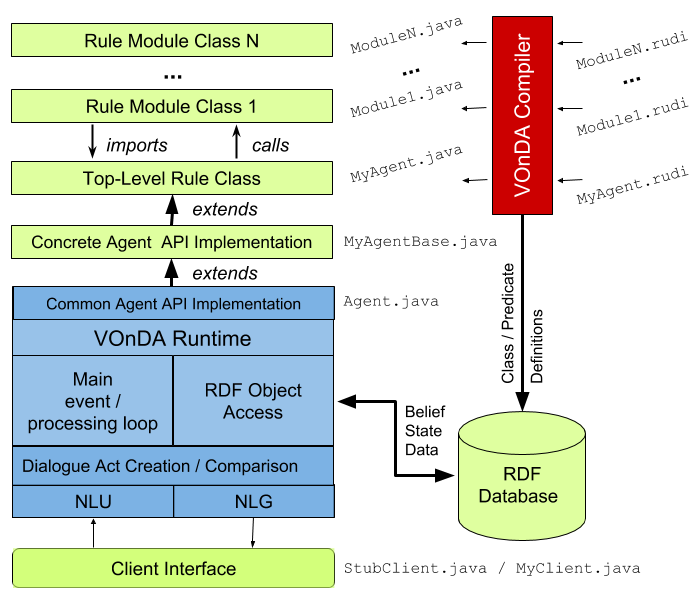
\includegraphics[width=.8\textwidth]{VOnDAStructureRot2.png}
  \caption{Gesamtarchitektur von Rudimant}
  \label{fig:architecture}
\end{figure}

%Rudimant besteht aus einem Compiler und einem Laufzeitsystem. Daraus wird eine
%konkrete Applikation, indem zunächst eine spezielle Java-Klasse, die sogenannte
%\emph{Wrapper-Klasse}, von der Klasse \texttt{Agent} abgeleitet wird. Diese
%kann Implementierungen von \texttt{Agent} erweitern oder
%überschreiben. Außerdem können eigene Java-Methoden für die Benutzung in den
%Regelfiles zur Verfügung stellen, die sich nicht ohne weiteres in \texttt{rudi}
%Dateien implementieren lassen (komplexe Queries an die Datenbank, etc.). Im
%Bild ist dies \texttt{MyAgent.java}.

A \vonda project consists of an ontology, a custom extension of the abstract
\texttt{Agent} class (the so-called \emph{wrapper class}), a client interface
to connect the communication channels of the application to the agent, and a
set of rule files that are arranged in a tree, using \texttt{import}
statements. The blue core in Figure~\ref{fig:architecture} is the run-time system that
is part of \vonda, while all green elements are the application specific parts
of the agent. A \texttt{Yaml} project file contains all necessary information
for compilation: the ontology, the wrapper class, the top-level rule file and
other parameters, like custom compile commands.

The \vonda compiler translates rule files with the extension \texttt{.rudi} to Java files. During this process, the ontology storing the RDF classes and properties is used to automatically infer types, resolve whether field accesses are actually accesses to the database, etc (see section \ref{sec:typeinference}).

Every rule file can define variables and functions in \vonda syntax which are
then available to all imported files.

The current structure assumes that most of the Java functionality that is used
inside the rule files will be provided by \texttt{Agent} superclass. There are,
however, alternative ways to use other Java classes directly.

The methods and fields from the custom wrapper class can be made available to all rule files by declaring them in the interface connecting the \texttt{.rudi} code to the Java framework. This interface must have the same name as the wrapper class but end with \texttt{.rudi} (in the example of figure ~\ref{fig:architecture}, this would be \texttt{MyAgent.rudi}).

%Damit der Compiler diese Funktionen kennt, müssen sie in der Datei
%\texttt{MyAgent.rudi} deklariert werden. Sie beschreibt sozusagen das
%Interface, auf das der \texttt{rudi} Quellcode zugreifen kann.

%\todo{Das kann man doch in allen .rudi files}
%Hier können auch statt der generischen Klasse \texttt{Rdf} die Klassen aus der
%Ontologie spezifiziert werden, wenn diese genauer angegeben werden können. Das
%hilft dem Kompiler bei der Typinferenz und dem richtigen Zugriff mit
%RDF-Prädikaten.

%Eine weitere wichtige Klasse ist \texttt{MyClient.java}, der die Kommunikation
%mit der Außenwelt herstellt und das Laufzeitsystem von konkreten
%Kommunikationsinterfaces abschirmt.


\subsection{The \vonda Rule Language}

%{\Huge TODO: testen, ob alle Beispiele so funktionieren, wie sie sollen !!!!!!}
\label{sec:language}

\if0
+ labeled rules
+ propose
  In the compiled code, the proposals are implemented as anonymous classes.
+ timeouts: for proactivity or monitoring on the side of the virtual agent
+ type inference
+ automatic transformation
+ intelligent boolean expressions
+ overloaded operators
+ functions
+ DA syntax

RDF store: HFC, probabilistic extensions (planned) ...
\fi

\vonda's rule language looks very similar to Java/C++. There are a number of
specific features which make it much more convenient for the specification of
dialogue strageties. One of the most important features is the way objects in
the RDF store can be used throughout the code: RDF objects and classes can be
treated similarly to those of object oriented programming languages, including
the type inference and inheritance that comes with type hierarchies.

%Die Klasse \texttt{MyAgent} inklusive Packagenamen muss in der config.yml Datei
%eines Projektes unter dem Eintrag \texttt{wrapperClass} spezifiziert werden, um
%im Compile-Schritt einen Effekt zu zeigen. Rudimant nutzt die Klasse
%\texttt{MyAgent} dann als Superklasse der im Compile-Schritt angegebenen Datei
%im rudi-Format und verlinkt Funktionsaufrufe und Variablennutzungen in allen
%untergeordneten rudi-Dateien auf diese, sodass korrekte Aufrufe im
%resultierenden Java-Code gewährleistet sind.


\subsubsection{The structure of a \vonda file}

%Anders als Java stellt rudimant nicht den Anspruch, dass die Einträge in einer
%Datei in irgendeine Form von übergeordneter Struktur gefasst werden. Die Regeln
%können ebenso wie Funktionsdeklarationen direkt in die Datei geschrieben
%werden. Dasselbe gilt für jede Art valider (Java-) Statements, wie etwa
%Zuweisungen, for-Schleifen usw.. Rudimant wird bei der Kompilation eine
%Java-Klasse erstellen, in die es die Funktionen sowie die Regeln, zu Funktionen
%transformiert, einträgt. Alle weiteren Statements werden in der korrekten
%Reihenfolge in die erzeugte Methode process() verschoben, wobei generierte
%Aufrufe an die Regelfunktionen zwischen ihnen gewährleisten, dass die Regeln
%und Statements in der Reihenfolge ausgeführt werden, die im rudi-Code
%spezifiziert war. Dies ermöglicht also, nicht in Regeln gefasste
%Abbruchbedingungen einzubauen, unter denen die Ausführung der ganzen Datei -
%und möglicher importierter Dateien - sofort beendet werden soll.
%
\vonda does not demand to group statements in some kind of high-level structure like e.g. a class construct. In fact, it is currently not possible to define classes in \texttt{.rudi} files at all. Rules and method declarations can just be put into the plain file. The same holds true for every kind of valid (Java-) statement, like assignments, for loops etc. From this basis, the compiler will create a Java class where the methods and rules that are transformed to methods are represented as the methods of this specific class. All other statements will be put into the \texttt{process()} method that \vonda creates to build a rule evaluation cycle. In doing so, the order of all statements (including the rules) is preserved.

This functionality offers possibilities to e.g. define and process high-level variables that you might want to have access to in all rules or to insert termination conditions that are not contained in rules.

%Datei-global deklarierte Variablen werden als Klassenvariablen angelegt.

\textbf{Warning:} It is important to know here that variables declared globally in a file will be transformed to fields of the Java class. We found that in very rare occasions, this can lead to unexpected behaviour when using them in a propose or timeout block as well as changing them in a global statement. As proposes and timeouts will not immediately be executed, they need every variable used inside them to be effectively final. \vonda leaves the evaluation of validness of variables for such blocks to Java. We found that Java might mistakenly accept variables that are not effectively final, what might lead to completely unexpected behaviour when proposes and timeouts with changed variable values are executed.

\subsubsection{RDF accesses and functional vs. relational properties}
\label{sec:rdfaccesses}

\begin{figure}[htb]
\begin{minipage}{0.5\columnwidth}
\small%
\begin{lstlisting}[language=Java]
user = new Animate;
user.name = "Joe";
set_age:
if (user.age <= 0) {
  user.age = 15;
}
\end{lstlisting}
\end{minipage}\ \vrule\hspace{1ex}
\begin{minipage}{0.44\columnwidth}
    \small\begin{tikzpicture}[
  blob/.style={circle, fill=yellow!50!white, minimum width=2mm},
  txt/.style={node distance=3mm}]
  \draw (0,0) node (agent) [blob]{};
  % BEWARE: RIGHT OF= IS DEPRECATED, DON'T USE IT
  \node (agtxt) [right= 0.1 of agent, txt] {Agent};
  \node (name) [below= 0.4 of agtxt.west, anchor=west]{\emph{name}: \texttt{xsd:string}};
  \node (animate) [blob, below=0.7 of agtxt.west]{};
  \node (antxt) [right= 0.1 of animate, txt] {Animate};
  \node (name) [below= 0.4 of antxt.west, anchor=west]{\emph{age}: \texttt{xsd:int}};
  \node (inanimate) [blob, below= 0.5 of animate, node distance=9mm]{};
  \node (intxt) [right= 0.1 of inanimate, txt] {Inanimate};
  \draw (agent) |- (animate);
  \draw (agent) |- (inanimate);
\end{tikzpicture}
\end{minipage}
  \caption{Ontology and \vonda code}
  \label{fig:rdfobjects}
\end{figure}

Figure \ref{fig:rdfobjects} shows an example of \vonda code, and how it relates
to RDF type and property specifications, schematically shown on the right.  The
domain and range definitions of properties are picked up by the compiler and
used in various places, e.g., to infer types, do automatic code or data
conversions, or create ``intelligent'' boolean tests, like in line 4, which
will expand into two tests, one testing for the existence of the property for
the object, and in case that succeeeds, a test if the value is greater than
zero. If there is a chain of more than one field/property access, every part is
tested for existence in the target code, keeping the source code as concise as
possible. Also for reasons of brevity, the type of a new variable needs not be
given if it can be inferred from the value assigned to it.

New RDF objects can be created with \texttt{new}, similar to Java objects; they
are immediately reflected in the database, as are all changes to already
existing objects.



\begin{table}[htbp]
  \centering
\begin{small}
\begin{minipage}[t]{0.35\textwidth}
\begin{lstlisting}[language=Java]
Child c;
String name = c.name;
c.name = "new name";
Set middle = c.middleNames;
c.middleNames += "John";
c.middleNames -= "James";
\end{lstlisting}
\end{minipage}
\begin{minipage}[t]{0.6\textwidth}
\begin{lstlisting}[language=Java]

String name = (String)c.getValue("<upper:name>");
c.setValue("<upper:name>", "new name");
Set middle = (Set<Object>)c.getValue("<upper:middleNames");
c.add("<upper:middleNames", "John");
c.remove("<upper:middleNames", "James");
\end{lstlisting}
\end{minipage}
\end{small}
  \caption{Examples for an RDF property access}
  \label{tab:property-access}
\end{table}
%\todo[inline]{missing creation of child in right row, plus "Set middle" is no proper code}

%Durch die Verbindung zu \texttt{hfc} während des Compile-Vorganges hat rudimant
%vollen Zugriff auf die Datenbank und kann nicht nur Rdf-Objekte anhand ihrer
%Typen erkennen, sondern auch erkennen, wann ein Feldzugriff auf ein Rdf-Objekt
%erfolgt und ihn in solchen Fällen in einen Zugriff auf die Datenbank
%umwandeln. Dies ist sowohl für Zugriffe auf Properties als auch für Änderungen
%ihres Inhalts möglich und lässt sich, sofern dies in der verwendeten Ontologie
%korrekt möglich ist, beliebig oft hintereinander ausführen.
%
Due to the connection of \vonda to HFC during compile time, it has full access to the database. Thereby, it cannot only recognize the correct RDF class to create a new instance from when encountering \texttt{new}, but it can also resolve property accessses to such instances. Field accesses as shown in line 2 and 3 of table \ref{tab:property-access} will be analyzed and transformed into database accessses. \vonda will also draw type information from the database. If the name property of the RDF class \texttt{Child} is of type String, exchanging line 2 by the line \texttt{int name = c.name} will result in a warning of the compiler.

In this process, the compiler will automatically recognize the equivalences of the following RDF and Java types:

\begin{figure}[h]
\small
\begin{lstlisting}[language=Java]
      {"<xsd:int>", "Integer"},
      {"<xsd:string>", "String"},
      {"<xsd:boolean>", "Boolean"},
      {"<xsd:double>", "Double"},
      {"<xsd:float>", "Float"},
      {"<xsd:long>", "Long"},
      {"<xsd:integer>", "Long"},
      {"<xsd:byte>", "Byte"},
      {"<xsd:short>", "Short"},
      {"<xsd:dateTime>", "Date"},
      {"<xsd:date>", "XsdDate"},
      {"<xsd:dateTimeStamp>", "Long"}
\end{lstlisting}
%\caption{Standard RDF types and the Java types as which they will be recognized}
\end{figure}

%Sowohl die Verwendung von relationalen als auch die von funktionalen Prädikaten
%ist erlaubt. Diese ändern die Aufrufe im rudi-Code jedoch grundsätzlich nicht,
%da rudimant selbst inferiert, ob ein Zugriff auf die Datenbank ein einfaches
%Objekt oder ein Set von Objekten zurückgibt. Lediglich die weitere Nutzung
%dessen, was abgerufen wurde, muss sich (selbstverständlich) an die Art des
%Ergebnisses des Rdf-Zugriffes anpassen. Versucht man allerdings, den Wert eines
%relationalen
%
Moreover, \vonda can see whether an access is done by functional or relational predicates and will handle it accordingly, deriving a collection type if necessary.

%Die beiden Operatoren \texttt{+=} und \texttt{-=} sind in rudimant
%überladen. Sie können sowohl wie in Java zum Rechnen mit Integer, float und
%double verwendet werden, als auch im Zusammenspiel mit Sets und
%Listen. \texttt{a += b} wird hierbei in \texttt{a.add(b)} umgewandelt,
%\texttt{a -= b} resultiert in \texttt{a.remove(b)}.

In the rule language, the operators \texttt{+=} and \texttt{-=} are overloaded. They can be used with sets and lists as shortcuts for adding and deleting objects. \texttt{a += b} will be compiled to \texttt{a.add(b)} and \texttt{a -= b} results in \texttt{a.remove(b)}.

\subsubsection{Rules and labels}

\begin{figure}
\begin{small}
\begin{lstlisting}[language=Java]
introduction:
  if (introduction){
    if (user.unknown){
      ask_for_name:
        if (talkative) {
          askForName();
        }
    } else {
      greetUser();
    }
  }
\end{lstlisting}
\end{small}
\caption{A simple rule}
\end{figure}

%Das Kernstück von rudimant sind die Dialogregeln. Eine Regel beginnt mit ihrem
%Namen, einem möglichst aussagekräftigen Label, gefolgt von einem
%Doppelpunkt. Anschließend folgt ein if-statement. Die Clause des Statements
%drückt die Bedingung aus, unter der die Regel ausgeführt werden soll, im Body
%steht der auszuführende Code.
%
The core of \vonda dialogue management are the dialogue rules, which will be evaluated in the run-time system on every environment trigger.

A rule starts with its name, from now on called label, followed by a colon. Pertaining to this label is an if-statement, possibly with else case. The clause of the if-statement expresses the condition under which the rule, or rather, the if block is to be executed; in the else block you can define what should happen if the rule cannot be executed, like stopping the evaluation of (a sub-tree of) the rules if necessary information is missing.

%Auch eingeschachtelte \texttt{if}-Abfragen können mit Labels versehen werden.
%Die Labels dienen einerseits zum debuggen des Codes, da im generierten Code
%Funktionalität enthalten ist, um den Agenten zur Laufzeit zu debuggen. Dazu
%kann man zur Zeit zwei API-Funktionen von \texttt{Agent} benutzen, nämlich
%\texttt{logRule(String rulename)} und \texttt{logAllRules()}
%
Rules can be nested to arbitrary depth, so if-statements inside a rule body can also be labelled. The labels are a valuable tool for debugging the life system, as they can be logged live with the debugger gui (cfg. chapter \ref{sec:debugger}). The debugger can show you which rules were executed when and what the individual results of each part of the conditions were.

%Der Output des Loggers wird dann das Label jeder Regel, die evaluiert wird,
%zusammen mit der Auswertung der Bedingung und den Werten aller booleschen
%Basisterme, die in der Bedingung vorhanden sind, angeben.

%For information on rule logging, see chapter \ref{sec:debugger}.
%\todo[inline]{Bsp debugging-output}

\subsubsection{Interrupting the rule evaluation cycle}

%Es gibt mehrere Möglichkeiten, die Regelverarbeitung lokal oder ganz
%abzubrechen. Aus einer gelabelten Regel kann man z.B. mit
%\verb|break label_name;| aussteigen. Alle danach folgenden Regeln werden dann
%weiter verarbeitet.
%
There are multiple ways to stop the rule evaluation locally (i.e. skipping the evaluation of the current subtree) or globally (i.e. stopping the whole evaluation cycle).

You can skip the evaluation of a specific rule you are currently in with the statement\verb|break label_name;|. This will only stop the rule with the respective label (no matter how deep the break statement is nested in it), such that the next following rule is evaluated next.

%Bricht man die Verarbeitung mit \texttt{cancel} ab, wird keine der in
%der Datei folgenden Regeln mehr angewandt, bei \texttt{cancel\_all} wird
%keine nachfolgende Regel, weder lokal, noch auf höheren Ebenen, angewandt.
%
If the evaluation is cancelled with the keyword \texttt{cancel;}, all of the following rules in the current file will be skipped (including any imported rules). If the keyword \texttt{cancel\_all} is used, none of the following rules, neither local nor higher in the rule tree, will be evaluated. This is the \vonda way of deciding not to evaluate whatever triggered the current evaluation cycle and should only be used as an 'emergency exit', as the dialogue rules should be rejecting any sound, non-matching trigger by themselves.

%Um \texttt{propose} oder \texttt{timeout} Blöcke zu verlassen, muss
%\texttt{return} benutzt werden, da dies normale Funktionsblöcke sind.

To leave \texttt{propose} and \texttt{timeout} blocks, you need to use an empty \texttt{return}, as they are only reduced representations of normal function bodies.

\subsubsection{\texttt{propose} and \texttt{timeout}}
\begin{figure}[htbp]
  \centering\small%
\begin{lstlisting}[language=Java]
if (!saidInSession(#Greeting(Meeting)) {
  // Wait 7 secs before taking initiative
  timeout("wait_for_greeting", 7000) {
    if (! receivedInSession(
              #Greeting(Meeting))
      propose("greet") {
        da = #InitialGreeting(Meeting);
        if (user.name)
          da.name = user.name;
        emitDA(da);
      }
  }

  if (receivedInSession(#Greeting(Meeting))
    // We assume we know the name by now
    propose("greet_back") {
      emitDA(#ReturnGreeting(Meeting,
                  name=\{user.name\});
    }
  }
}
\end{lstlisting}\vspace*{-3ex}
  \caption{\vonda code example}
  \label{fig:propose}
\end{figure}

There are two statements with a special syntax and semantics: \texttt{propose}
and \texttt{timeout}. \texttt{propose} is \vonda's current way of implementing
probabilistic selection. All (unique) propose blocks that are in active rule
actions are collected, frozen in the execution state in which they were
encountered, like closures known from functional programming languages. When
all possible proposals have been selected, a statistical component decides
which one will be taken and the closure is executed.

\texttt{timeout}s also generate closures, but with a different purpose. They
can be used to trigger proactive behaviour, or to check the state of the system
after some time period, or in regular intervals. A timeout will only be created
if there is no active timeout with that name.

\subsubsection{Dialogue acts}
%\subsubsection{Dialogue acts, their evaluation and "real" variables}
\label{sec:caret}

%Eine wichtige Aufgabe eines Dialogsystems ist zweifellos die Ausgabe von
%Dialogakten, die von der Generierungskomponente zu Kommunikation mit dem Nutzer
%verarbeitet werden können. In rudimant ist die Funktion \texttt{emitDA} hierfür
%zuständig.

Without doubt, an important task of a dialogue system is emitting dialogue acts that can be transformed to natural language by the generation component to communicate with the user. In \vonda, the function responsible for this is \texttt{emitDA}.

The dialogue act representation is an internal feature of \vonda. We are currently using the DIT++ dialogue act hierarchy \citep{bunt2012iso} and shallow frame semantics along the lines of FrameNet \citep{ruppenhofer2016framenet} to represent dialogue acts. The natural language understanding and generation units connected to \vonda should therefore be able to generate or, respectively, process this representation.
%interface with the natural language understanding and generation units.
% While shallow semantics is enough for most applications, we already experience its shortcomings when trying to handle, for example, social talk.

\begin{figure}[htb]
  \centering\small%
\begin{lstlisting}[language=Java]
emitDA(#Inform(Answer, what={solution}));
\end{lstlisting}\vspace*{-3ex}
  \caption{\vonda code example}
  \label{fig:DA}
\end{figure}

%Figure~\ref{fig:DA} contains an example of the short-hand notation
%for shallow semantic structures (starting with \textbf{\texttt{\#}}).  Since
%they predominantly contain constant (string) literals, this is the default when
%specifying such structures. The special ``hat'' syntax in
%\texttt{user=\^{}user.name} allows to insert the value of expressions into the
%literal, similar to an \emph{eval}.

%Argument von \texttt{emitDA} ist ein Dialogakt in der oben gezeigten Form. Dass
%es sich bei \texttt{Inform}\verb|(...)| nicht um einen Funktionsaufruf, sondern
%um einen Dialogakt handelt, wird hier und an allen anderen Stellen, an denen
%man einen Dialogakt benutzen möchte, durch das \verb|#|
%gekennzeichnet. Rudimant wird so erkennen, dass im Java-Code eine neue Instanz
%der Klasse DialogueAct mit den entsprechenden Modifikationen erstellt werden
%muss. Hierbei kommt dem Marker \caret{} eine besondere Bedeutung zu: Per
%default werden alle in den Klammern angegebenen Argumente, egal, ob sie rechts
%oder links eines $=$ stehen, als Strings an den neuen DialogueAct
%übergeben. Möchte man explizit den Inhalt einer Variablen oder eines Ausdrucks
%übergeben, so ist die Benutzung von \caret{} vor der entsprechenden rechten
%Seite einer Zuweisung notwendig, die dafür sorgt, dass der Ausdruck evaluiert
%wird, und nicht als atomares Symbol interpretiert.

The dialogue act passed to \texttt{emitDA} should look as shown in figure \ref{fig:DA}. \texttt{Inform}\verb|(...)| will be recognized by \vonda as dialogue act because it has been marked with \verb|#|. It will then create a new instance of the class DialogueAct that contains the respective modifications. As a default, arguments of a DialogueAct creation (i.e., character strings on the left and right of $=$) are seen as and transformed to constant (string) literals, because most of the time that is what is needed.
%The special ``hat'' syntax with \caret allows to mark when the following string is a real variable or an expression and should be evaluated.
Surrounding a character sequence with curly brackets (\{\}) marks it as an
expression that should be evaluated, in fact, arbitrary expressions are allowed
inside the curly brackets.

\subsubsection{Type inference and overloaded operators}
\label{sec:typeinference}

%Rudimant erlaubt statische Typzuweisungen sowie Casting, beides ist jedoch
%nicht zwingend notwendig.
%
\vonda allows static type assignments and casting, but neither of them is always necessary.

%Ist beispielsweise der Typ der rechten Seite einer Variablendeklaration mit
%Zuweisung bekannt oder inferierbar, so ist es nicht notwendig, den Typ der
%Variablen explizit anzugeben.

If, for example, the type of the expression on the right-hand side of declaration assignment is known or inferrable, it is not necessary to explicitely state it.

You can also declare variables final.

\begin{table}[htbp]
  \centering
  \begin{small}
    \begin{lstlisting}[language=Java]
      if (! c.user.personality.nonchalance){ ... }
    \end{lstlisting}

    {\Large$\Downarrow$}\\

    \begin{lstlisting}[language=Java]
      if (!((((c != null) && (c.user != null))
             && (c.user.personality != null))
            && (c.user.personality.nonchalance != null))) {
         ...
      }
\end{lstlisting}
\end{small}

\caption{Transformation of complex boolean expressions}
\label{tab:multi-predaccess}
\end{table}
\vspace*{10pt}

%Als zeitsparendes Feature bietet rudimant insbesondere das automatische
%Vervollständingen von bool'schen Ausdrücken in den Clauses von if, while und
%for an. Da in diesem Fall bekannt ist, dass das Ergebnis boolean sein muss,
%ergänzt rudimant automatisch den Test auf die Existenz eines Objektes in der
%Clause, sollte dieses nicht Typ boolean sein. Bei Feldzugriffen testet es für
%jeden Teilzugriff, dass das erhaltene Objekt nicht null ist, um einer
%NullPointerException zur Laufzeit des generierten Codes vorzubeugen.

A time-saving (and code-readability-improving) feature of \vonda is the automatic completion of boolean expressions in the clauses of if, while and for statements. As it is obvious in these cases that the result of the expression must be of type boolean, \vonda automatically fills in a test for existence if it is not boolean. When encountering field accesses, it makes sure that every partial access is tested for existence (i.e., not \texttt{null}) to avoid a NullPointerException in the runtime execution of the generated code.

%Die Vergleichsoperatoren in rudimant sind überladen. Neben den aus Java bekannten Anwendungen als Vergleichsoperatoren können sie auch auf Dialogakte angewendet werden. In diesen Fällen werden sie zu Subsumptionsoperatoren.

Many operators are overloaded, especially boolean operators such as
\textbf{\texttt{<=}}, which compares numeric values, but can also be used to test if an
object is of a specific class, for subclass tests between two classes, and for
subsumption of dialogue acts.

\begin{table}[htbp]
  \centering
  \begin{footnotesize}
    \begin{minipage}{0.3\textwidth}
\begin{lstlisting}[language=Java]
if (sa <= #Question){
  ...
}
\end{lstlisting}
    \end{minipage}
    \begin{minipage}{0.5\textwidth}
\begin{lstlisting}[language=Java]
if (sa.isSubsumedBy(new DialogueAct("Question")) {
  ...
}
\end{lstlisting}
    \end{minipage}
  \end{footnotesize}

  \caption{Overloaded comparison operators}
  \label{tab:overloaded-comparison}
\end{table}

%\paragraph{Rudimant Typinformationen zur Verfügung stellen}
\subsubsection{External methods and fields}
\label{sec:javatypes}

As mentioned before, you can use every method or field that you declare in your custom Agent implementation in your \vonda code. Their declaration in the Java-rudi interface should look like a normal Java field or method definition (cfg. figure \ref{tab:javadef}). It is possible to use generics in these definitions, although they are, for complexity reasons, restricted to be one single uppercase letter.

\begin{table}[htbp]
  %\centering
  \small
  \begin{tabular}{lp{.45\textwidth}}
    \begin{lstlisting}[language=Java]
    myType someVariable;
    \end{lstlisting}
    &  there is a variable of type \texttt{myType} \\

    \begin{lstlisting}[language=Java]
    myType someFunction(typeA a, typeB b);
    \end{lstlisting}
    &  the method someFunction takes arguments of types \texttt{typeA} and
      \texttt{typeB} and returns an object of type \texttt{myType} (void =
      void)
  \end{tabular}

  \caption{Defintions of existing Java fields and methods for \vonda}
  \label{tab:javadef}
\end{table}

There is a variety of standard Java methods called on Java classes that \vonda automatically recognizes, like e.g. the substring method for Strings. If you find that you need \vonda to know the return type of a new method that can or should only be called upon instances of a specific class, you can provide \vonda with knowledge about them by adding their definition to the interface as follows:


\begin{table}[htbp]
  \centering
  \small
  \begin{tabular}{lp{.45\textwidth}}

    \begin{lstlisting}[language=Java]
     [type]. myType Function(typeA a);
    \end{lstlisting}
    & declaration of a function that has to be called on an instance of class \texttt{type}.
  \end{tabular}

  \caption{Definition of a non-static method of Java objects}
  \label{tab:methoddef}
\end{table}

Of course you can also use generics in these definitions. For example, the get method on lists is defined as follows in the \vonda framework:

\begin{figure}[htbp]
\centering
\small
\begin{lstlisting}[language=Java]
 [List<T>]. T get(int a);
\end{lstlisting}
\end{figure}
%Für Funktionen, die nicht oder nur umständlich in rudi-Code implementiert
%werden können, sollte der Nutzer eine Javaklasse \texttt{MyAgent} von der
%abstrakten Klasse \texttt{Agent} ableiten. Diese Klasse wird als
%\emph{Wrapper-Klasse} bezeichnet. Funktionen und Variablen, die in
%dieser Klasse deklariert wurden und später im rudi-Code benutzt werden sollen,
%müssen mit vollständiger Typangabe in einer Datei \texttt{MyAgent.rudi}
%deklariert werden, sodass die Typinferenz von rudimant sie korrekt
%berücksichtigen kann (zur Syntax siehe \ref{sec:rudimant-Typinferenz}).
%

%In manchen Fällen, wie etwa der Benutzung von außerhalb der rudi-Dateien
%deklarierten Funktionen und Variablen, ist es notwendig, rudimant Informationen
%über Typen zu geben. Dabei gilt folgendes Schema, nach dem Typen an beliebiger
%Stelle, für gewöhnlich jedoch in der Datei MyAgent.rudi (siehe
%\ref{rudimant-global}) deklariert werden können:

It is important to realize that whatever declarations are in the interface are only compile information for \vonda and will not be transferred to the compiled code, whereas such declarations in the rule code itself will also appear in the compiled code.

%Wichtig ist: Diese Deklarationen werden nur für die Berechnung der Typen durch
%rudimant angegeben und werden nicht in den kompilierten Code
%übernommen. Insbesondere Zeilen wie \texttt{int i;} oder \texttt{void
%  someFunction();} entsprechen damit nicht einer gleich aussehenden Deklaration
%im Java-Code. Falls es einen Grund geben sollte, dass die Zeilen als im
%Compile-Ergebnis als dringend erforderlich betrachtet werden, hilft die in
%Kapitel \ref{rudi-verbatim} beschriebene Methode.

%\subsubsection{Überladene Vergleichsoperatoren und Tests}
%Dies überschneidet sich in großen Teilen mit dem Doku-Teil zur Typinferenz; wurde dort untergebracht

\subsubsection{Functional constructs}

%Rudimant erlaubt die Verwendung von lambda-Konstrukten. Im moment können sie
%aber nur für die Implementierung von \texttt{Predicate}
%resp. \texttt{Comparator} in den im folgenden angegebenen vier
%Funktionen. Diese Funktionen sind in \texttt{Agent} vordefiniert. Ein
%einfaches Beispiel zum Filtern von Objekten mit einer Subtyprelation wäre:

\vonda allows for using lambda constructions. At the moment, their usage is limited to the implementation of \texttt{Predicate} or \texttt{Comparator} in the following functions that are pre-defined in the Agent framework.

\begin{table}[htbp]
  \centering
  \begin{small}
\begin{lstlisting}[language=Java]
boolean contains(Collection coll, Predicate pred);
boolean all(Collection coll, Predicate pred);
List<Object> filter(Collection coll, Predicate pred);
List<Object> sort(Collection coll, Comparator c);
\end{lstlisting}
  \end{small}

  \caption{Functions that take lambda expressions as an argument}
  \label{tab:lambda-functions}
\end{table}

For example, if you want to filter a set of RDF objects by a subtype relation, you can write:

\begin{lstlisting}[language=Java]
des = filter(agent.desires, (d) -> ((Desire)d) <= UrgentDesire);
\end{lstlisting}

\subsubsection{\texttt{import}}

%\texttt{import} ist ein Schlüsselwort in rudimant. Eine Zeile ''\texttt{import
%  File;}'' auf globaler Ebene, an einer beliebigen Stelle zwischenn den Regeln,
%bedeutet die Inklusion der Datei File.rudi an exakt dieser Stelle. Hiermit wird
%zum einen erreicht, dass rudimant auch diese Datei zu ausführbarem Java-Code
%kompiliert, sodass nicht alle Dateien eines Projektes separat kompiliert werden
%müssen. Zum anderen wird das vollständige Regelinventar der Datei an der
%entsprechenden Stelle im Java-Code mithilfe ihrer process-Methode aufgerufen
%und durchgearbeitet.
%
\texttt{import} is a keyword in the \vonda language. A global line like ''\texttt{import File;}'', to be placed at an arbitrary positions between the rules, results in the inclusion of the file \texttt{File.rudi} at exactly this position.

This inclusion has two important effects. On one side, it triggers the compilation of the included file at exact this point, such that any fields and methods known at this time will be available in the important file and it does not need to be compiled seperately. On the other side, it has the effect that all the rules contained in the important file will be inserted in the rule cycle at the specific point of the \texttt{import}, where in the resulting code the \texttt{process()} method of the imported file will be executed.

%\texttt{import} ermöglicht es also, das Regelinventar für ein Projekt auf
%mehrere Dateien bzw. mehrere Module aufzuteilen und diese zusammenzustecken,
%sodass ein einziger Aufruf ausreicht, um sie zu kompilieren und später auch, um
%die Auswertung der Regeln anzustoßen. Dies ist nicht nur nützlich zur
%Übersichtlichkeit und Strukturierung des Projektes, sondern fördert auch die
%Modularität, da verschiedene 'Unterbäume' der \texttt{import}-Hierarchie leicht
%ausgeklinkt oder aus anderen Projekten wiederverwendet werden können.

So the \texttt{import} functionality make sit possible to distribute the rules of a project into multiple files, respectively modules, and pin them together in such a way that they are handled as one unit when compiling or executing the compilied code. This is not only useful for clarity and structuring of project, but also supports modularity, as different subtrees of the \texttt{import} hierarchy can easily be added, moved, taken away or re-used in different projects.

\subsubsection{Java-Code verbatim in rule files} \label{sec:rudi-verbatim}

%Rudimant verarbeitet eine Regelsprache, die mit voller Absicht nur
%eingeschränkte Java-Funktionalitäten zur Verfügung stellt. Was in rudi-Code
%nicht umzusetzen ist, sollte in Funktionen in die übergeordnete Java-Klasse
%wandern (vgl. \ref{rudimant-global}).
%
To maintain simplicitely, \vonda intentionally only provides limited Java functionalities. Whatever is not feasible in \texttt{.rudi} code should be done in methods in the wrapper class (cfg. \ref{rudimant-global}).

%Für Fälle, in denen dies nicht genügt und vor Ort eine Funktionalität benötigt
%wird, die rudimant nicht parsen oder nicht richtig darstelllen kann, ist eine
%verbatim-Umgebung vorgesehen. Alles, was innerhalb der Zeichenfolgen \verb|/*@|
%und \verb|@*/| steht, wird behandelt wie ein mehrzeiliges Java-Kommentar, wird
%also in genau diesem Aussehen in den resultierenden Code übertragen. Dabei
%werden die klammernden Zeichenfolgen ausgelassen.
%
In cases where this is not enough and you urgently need a functionality in a \texttt{.rudi} file that \vonda cannot parse or represent correctly, you can use its verbatim funciton. Everything between \verb|/*@| and \verb|@*/| will be treated like a multi-line Java comment, meaning the content is not parsed or evaluated further. It will be transferred to the compiled code at exactly this position between statements, but without the comment symbols.

%Diese Funktionalität kann insbesondere dazu benutzt werden, am Anfang einer
%\texttt{rudi} Datei Java-Klassen zu importieren, die im kompilierten Code
%gebraucht werden.

In particular, this functionality can be used to import Java classes at the beginning of a rule file. You should however be aware that \vonda will not know these classes nor their methods and fields. It will however accept creations of instances of unknown classes, as well as your casting of results of unknown methods. If, be it for commodity or for other reasons, you want \vonda to have type information about methods called on instances on one of these classes, you can put this information into the type interface of the wrapper class (cfg. chapter \ref{sec:javatypes}).

\section{The Run-Time System}
%\subsection{Run-Time Library}

The run-time library contains the basic functionality for handling the rule
processing, including the proposals and timeouts, and for the on-line
inspection of the rule evaluation. There is, however, no blueprint for the main
event loop, since that depends heavily on the host application. It also
contains methods for the creation and modification of shallow semantic
structures, and especially for searching the interaction history for specific
utterances. Most of this functionality is available through the abstract
\texttt{Agent} class, which has to be extended to a concrete class for each
application.

There is functionality to talk directly to the HFC database using queries, in
case the object view is not sufficient or to awkward. The natural language
understanding and generation components can be exchanged by implementing existing
interfaces, and the statistical component is connected by a message exchange
protocol. A simple generation engine based on a graph rewriting module is
already integrated, and is used in our current system as a template based
generator. The example application also contains a VoiceXML based
interpretation module.

A set of reactive rules is executed whenever there is a change in the
information state (IS). These changes are caused by incoming sensor or
application data, intents from the speech recognition, or expired timers.
Rules are labeled if-then-else statements, with complex conditions and shortcut
logic, as in Java or C. The compiler analyses the base terms and stores their
values during processing for dynamic logging. A rule can have direct effects,
like changes in the IS, or system calls. Furthermore, it can generate so-called
\emph{proposals}, which are (labeled) blocks of code in a frozen state that
will not be immediately executed, similar to closures.

All rules are repeatedly applied until a fix point is reached: No new proposals
are generated and there is no IS change in the last iteration. Then, the set of
proposals is evaluated by a statistical component, which will select the best
alternative. This component can be exchanged to make it as simple or elaborate
as necessary, taking into account arbitrary features from the data storage.

\subsection{Functionalities (methods) Provided by the Run-Time System}
%Alles was in \texttt{Agent} bereitgestellt wird. Die aktuelle Liste der
%bereitgestellten Funktionen finden sich in \texttt{rudimant} unter
%\texttt{src/main/resources/Agent.rudi}.
The following methods are declared in \texttt{src/main/resources/Agent.rudi} and implemented in the \vonda framework.

\begin{itemize}
\item Pre-added Java methods
\begin{lstlisting}[language=Java]
[Object]. boolean equals(Object e);
[String]. boolean startsWith(String s);
[String]. boolean endsWith(String s);
[String]. String substring(int i);

[List<T>]. T get(int a);
[Collection<T>]. void add(Object a);
[Collection<T>]. boolean contains(Object a);
[Collection<T>]. int size();
\end{lstlisting}

\item Short-hand conversion methods from Agent
\begin{lstlisting}[language=Java]
int toInt(String s);
float toFloat(String s);
double toDouble(String s);
boolean toBool(String s);
\end{lstlisting}

\item Other Agent methods
\begin{lstlisting}[language=Java]
// Telling the Agent that something changed
void newData();

String getLanguage();

// Math methods
int random(int limit);
float random();

// logging methods
Logger logger;

// discarding actions and shutdown
void clearBehavioursAndProposals();
void shutdown();
\end{lstlisting}

\item Timeouts
\begin{lstlisting}[language=Java]
void newTimeout(String name, int millis);
boolean isTimedOut(String name);
void removeTimeout(String name);
boolean hasActiveTimeout(String name);
// cancel and remove an active timeout, will not be executed
void cancelTimeout(String name);
\end{lstlisting}

\item Methods handling with dialogue acts
\begin{lstlisting}[language=Java]
// sending of dialogue acts
DialogueAct createEmitDA(DialogueAct da);
DialogueAct emitDA(int delay, DialogueAct da);
DialogueAct emitDA(DialogueAct da);

// Access to dialogue acts of the current session
// my last outgoing resp. the last incoming dialogue act
DialogueAct myLastDA();
DialogueAct lastDA();

// did i say something like ta in this session (subsumption)? If so, how many
// utterances back was it? (otherwise, -1 is returned)
int saidInSession(DialogueAct da);
// like saidInSession, only for incoming dialogue acts
int receivedInSession(DialogueAct da);

boolean waitingForResponse();
void lastDAprocessed();
DialogueAct addLastDA(DialogueAct newDA);
[DialogueAct]. void setProposition(String prop);
\end{lstlisting}

\item Methods using lambda expressions
\begin{lstlisting}[language=Java]
// lambda: first class argument of Function is return type of function object
boolean contains(Collection<T> coll, Function<Boolean, T> pred);
boolean all(Collection<T> coll, Function<Boolean, T> pred);
List<T> filter(Collection<T> coll, Function<Boolean, T> pred);
List<T> sort(Collection<T> coll, Function<Integer, T, T> c);
Collection<T> map(Collection<S> coll, Function<T, S> f);
\end{lstlisting}

\end{itemize}

%%% Local Variables:
%%% mode: latex
%%% TeX-master: "userguide"
%%% End:
